%%%%%%%%%%%%%%%%%%%%%%%%%%%%%%%%%%%%%%%%%%%%%%%%%%%%%%%%%%%%%%%%%%%%%%%
%% DOKUMENTVORLAGE THOMAS DIETRICH  %%%%%%%%%%%%%%%%%%%%%%%%%%%%%%%%%%%
%%%%%%%%%%%%%%%%%%%%%%%%%%%%%%%%%%%%%%%%%%%%%%%%%%%%%%%%%%%%%%%%%%%%%%%


%%%%%%%%%%%%%%%%%%%%%%%%%%%%%%%%%%%%%%%%%%%%%%%%%%%%%%%%%%%%%%%%%%%%%%%
%% SSE Thesis Document Template (Thomas Dietrich) %%%%%%%%%%%%%%%%%%%%%
%%%%%%%%%%%%%%%%%%%%%%%%%%%%%%%%%%%%%%%%%%%%%%%%%%%%%%%%%%%%%%%%%%%%%%%

\documentclass[
		12pt,						% font size
		english,					% english document
		%ngerman,					% deutsches Dokument, f�r Umlaute, Silbentrennung etc. (Umlauts, Hyphenation)
		a4paper,					% paper size
		%oneside,					% single-sided document
		twoside,					% two-sided document
		titlepage,					% the title page is used (will start right)
		parskip=half,				% space between paragraphs (half line)
		headings=normal,			% decrease size of headers
		open=right,					% chapter beginnen rechts
		listof=totoc,				% list directories in the table of contents
		bibliography=totoc,			% list bibliography in the table of contents
		captions=tableheading,		% output labeling tables below
		draft=false, 				% draft=true useful during writing, set to false for final document
]{scrreprt}
%%%%%%%%%%%%%%%%%%%%%%%%%%%%%%%%%%%%%%%%%%%%%%%%%%%%%%%%%%%%%%%%%%%%%%%


%% Scripture and Language %%%%%%%%%%%%%%%%%%%%%%%%%%%%%%%%%%%%%%%%%%%%%
\usepackage[english]{babel}
%\usepackage[ngerman]{babel}
\usepackage[T1]{fontenc}
\usepackage[ansinew]{inputenc}
\usepackage{textcomp} % Euro-Sign etc.
\usepackage{lmodern}

%\usepackage[T1]{fontenc}
%\usepackage[utf8x]{inputenc}
%\usepackage{libertine}
%\usepackage[ngerman]{babel}

%\usepackage{xunicode}
%\usepackage{fontspec}
%\usepackage{xltxtra} % For XeLaTeX
%\setromanfont[Mapping=tex-text]{Linux Libertine O}		% serif font
%\setsansfont[Mapping=tex-text]{Linux Biolinum O}		% sanserif font
%\setmonofont[Mapping=tex-text,Scale=0.9]{Courier New}	% font for code
%\setmonofont[Mapping=tex-text]{DejaVu Sans Mono}
%\usepackage{polyglossia}
%\setdefaultlanguage[spelling=new,latesthyphen=true]{english}
%%%%%%%%%%%%%%%%%%%%%%%%%%%%%%%%%%%%%%%%%%%%%%%%%%%%%%%%%%%%%%%%%%%%%%%


%% Global Document Information %%%%%%%%%%%%%%%%%%%%%%%%%%%%%%%%%%%%%%%%
\newcommand{\thesistitle}{Thesis Title}
\newcommand{\thesistype}{Master Thesis}
\newcommand{\autor}{Author Name}
\newcommand{\mail}{author-email@tu-ilmenau.de}
\newcommand{\courseofstudies}{rocket science}
\newcommand{\matriculationnr}{XXXXX}
\newcommand{\supervisor}{Prof. Responsible}
%\newcommand{\secondtutor}{Second Reader}
\newcommand{\faculty}{Department of Computer Science and Automation}
\newcommand{\department}{Systems and Software Engineering Group}
\newcommand{\location}{Ilmenau}
\newcommand{\registrationdate}{XX.~January 20XX}
\newcommand{\submissiondate}{XX.~June 20XX}
\newcommand{\submissiontimestamp}{XX.XX.20XX}
%%%%%%%%%%%%%%%%%%%%%%%%%%%%%%%%%%%%%%%%%%%%%%%%%%%%%%%%%%%%%%%%%%%%%%%


%% Graphics & Illustrations %%%%%%%%%%%%%%%%%%%%%%%%%%%%%%%%%%%%%%%%%%%
\usepackage{graphicx}			% in order to load graphics
\usepackage{wrapfig}			% integration of graphics with wraping text
\usepackage{subfig}				% integration of multiple objects within a float
\usepackage{pdfpages}			% binds a graphic or page (.pdf or .jpg) in the document
\usepackage{float}
\graphicspath{{images/}}
%%%%%%%%%%%%%%%%%%%%%%%%%%%%%%%%%%%%%%%%%%%%%%%%%%%%%%%%%%%%%%%%%%%%%%%


%% Directory Definition %%%%%%%%%%%%%%%%%%%%%%%%%%%%%%%%%%%%%%%%%%%%%%%
%\usepackage{tikz}
%\usetikzlibrary{trees}
%\usepackage{xcolor}
\usepackage{dirtree}
%%%%%%%%%%%%%%%%%%%%%%%%%%%%%%%%%%%%%%%%%%%%%%%%%%%%%%%%%%%%%%%%%%%%%%%


%% Input Text Files %%%%%%%%%%%%%%%%%%%%%%%%%%%%%%%%%%%%%%%%%%%%%%%%%%%
%\usepackage[dvipsnames]{xcolor}
\usepackage{fancyvrb}

% redefine \VerbatimInput
\RecustomVerbatimCommand{\VerbatimInput}{VerbatimInput}%
	{fontsize=\footnotesize,
	%
	frame=lines,  % top and bottom rule only
	framesep=2em, % separation between frame and text
	rulecolor=\color{gray},
	%
	%label=\fbox{\color{black}data.txt},
	labelposition=topline,
	%
	commandchars=\|\(\), % escape character and argument delimiters for commands within the verbatim
	commentchar=*        % comment character
}
%%%%%%%%%%%%%%%%%%%%%%%%%%%%%%%%%%%%%%%%%%%%%%%%%%%%%%%%%%%%%%%%%%%%%%%


%% Line Spacing and Margins %%%%%%%%%%%%%%%%%%%%%%%%%%%%%%%%%%%%%%%%%%%
\usepackage{setspace}
\usepackage{geometry}
%%%%%%%%%%%%%%%%%%%%%%%%%%%%%%%%%%%%%%%%%%%%%%%%%%%%%%%%%%%%%%%%%%%%%%%


%% Bibliography %%%%%%%%%%%%%%%%%%%%%%%%%%%%%%%%%%%%%%%%%%%%%%%%%%%%%%%
\usepackage[numbers,square]{natbib}
\bibliographystyle{alphadin}
%\bibliographystyle{alpha}
%\bibliographystyle{siam}
%\bibliographystyle{apalike}
%\bibliographystyle{acm}    % [1], APP, N, alfabetico
%\bibliographystyle{phjcp}  % [1], N. APP, aparicion
%%%%%%%%%%%%%%%%%%%%%%%%%%%%%%%%%%%%%%%%%%%%%%%%%%%%%%%%%%%%%%%%%%%%%%%


%% TODOs %%%%%%%%%%%%%%%%%%%%%%%%%%%%%%%%%%%%%%%%%%%%%%%%%%%%%%%%%%%%%%
%\usepackage{pdfcomment}
\usepackage[%
		%disable,
		english,
		%german,
		textsize=tiny,
		colorinlistoftodos
]{todonotes}
\newcommand{\todoref}[1]{\todo[color=blue!40]{Missing Reference #1}}
\newcommand{\todoedit}[1]{\todo[color=green!40]{#1}}
%%%%%%%%%%%%%%%%%%%%%%%%%%%%%%%%%%%%%%%%%%%%%%%%%%%%%%%%%%%%%%%%%%%%%%%


%% HyperRef %%%%%%%%%%%%%%%%%%%%%%%%%%%%%%%%%%%%%%%%%%%%%%%%%%%%%%%%%%%
% http://www.tug.org/applications/hyperref/manual.html
\usepackage[
		pdftitle={\thesistitle},	% Sets the document information Title field
		pdfauthor={\autor},			% Sets the document information Author field
		pdfsubject={\thesistype},	% Sets the document information Subject field
		%backref=section,			% Adds backlink text to the end of each item in the bibliography, as a list of section numbers
		%pdfpagelabels,
		pdfpagelayout=TwoColumnRight,
		%pdfpagelayout=TwoPageRight, % Displays two pages, odd-numbered pages to the right % Attention, PDF-Version 1.5 required
		%pdfdisplaydoctitle=true,	% Display document title instead of file name in title bar
		hypertexnames=false,		% To properly display the bookmarks
		%linktocpage 				% Social bookmarking numbers instead of text in the table of contents
		bookmarks,
		bookmarksnumbered=true,
		bookmarksopen=true,
		bookmarksopenlevel=1,
		hyperfootnotes=false,
		%unicode=true,
		colorlinks=true,
		
	%% These color definitions should be used for printing (all black)
	%	linkcolor=black, 		% Simple internal links
	%	anchorcolor=black, 		% Anchor text
	%	citecolor=black, 		% References to the bibliography entries in text
	%	filecolor=black, 		% Shortcuts, open local files
	%	menucolor=black, 		% Acrobat menu items
	%	urlcolor=black, 		% Color of external URLs linked text
	%% These color definitions can be used for distribution in PDF or for colored printing
		linkcolor=darkblue,		% Simple internal links
		citecolor=darkblue, 	% References to the bibliography entries in text
		menucolor=darkblue,		% Acrobat menu items
		urlcolor=cyan, 			% Color of external URLs linked text
]{hyperref}

% Link URL, long URLs wrap etc.
\usepackage{url}
%%%%%%%%%%%%%%%%%%%%%%%%%%%%%%%%%%%%%%%%%%%%%%%%%%%%%%%%%%%%%%%%%%%%%%%


%% Paragraph Settings %%%%%%%%%%%%%%%%%%%%%%%%%%%%%%%%%%%%%%%%%%%%%%%%%
%\setlength{\parskip}{3pt}
%\setlength{\parindent}{0pt}
%%%%%%%%%%%%%%%%%%%%%%%%%%%%%%%%%%%%%%%%%%%%%%%%%%%%%%%%%%%%%%%%%%%%%%%


%% Abbreviations %%%%%%%%%%%%%%%%%%%%%%%%%%%%%%%%%%%%%%%%%%%%%%%%%%%%%%
\usepackage[intoc]{nomencl}
\let\abbrev\nomenclature
%\renewcommand{\nomname}{Abk�rzungsverzeichnis}
\renewcommand{\nomname}{Abbreviations}
\setlength{\nomlabelwidth}{.25\hsize}
\renewcommand{\nomlabel}[1]{#1 \dotfill} % dots between abbreviations and explainations
\setlength{\nomitemsep}{-\parsep} % Decrease line spacing
%%%%%%%%%%%%%%%%%%%%%%%%%%%%%%%%%%%%%%%%%%%%%%%%%%%%%%%%%%%%%%%%%%%%%%%


%%%%%%%%%%%%%%%%%%%%%%%%%%%%%%%%%%%%%%%%%%%%%%%%%%%%%%%%%%%%%%%%%%%%%%%
\usepackage{siunitx}
\sisetup{
	%locale=UK,
	%locale=US,
	locale=DE,
	load-configurations=binary,
	load-configurations=abbreviations,
	per-mode=symbol,
}
\DeclareSIUnit\bit{Bit}
\DeclareSIUnit\byte{Byte}
% Usage:
%	\SI[options]{value}[pre-unit]{unit}
%	\si[options]{unit}
%	\num[options]{number}
%	\ang[options]{angle}
%%%%%%%%%%%%%%%%%%%%%%%%%%%%%%%%%%%%%%%%%%%%%%%%%%%%%%%%%%%%%%%%%%%%%%%


%% more featurerich and modern tables %%%%%%%%%%%%%%%%%%%%%%%%%%%%%%%%%
\usepackage{booktabs}
\setlength{\belowbottomsep}{\belowrulesep} % replaces 0pt-distance between bottomrule and caption
%\renewcommand*{\arraystretch}{1.2} more space between rows
% Usage:
%   \toprule, \midrule, \bottomrule
%   \cmidrule, \addlinespace
%%%%%%%%%%%%%%%%%%%%%%%%%%%%%%%%%%%%%%%%%%%%%%%%%%%%%%%%%%%%%%%%%%%%%%%


%% Miscellaneous %%%%%%%%%%%%%%%%%%%%%%%%%%%%%%%%%%%%%%%%%%%%%%%%%%%%%%
\usepackage{ifdraft}					% run depending on draft or final in documentclass % \ifdraft{draft case}{final case}
\usepackage{amsmath,amssymb,amstext} 	% For mathematical symbols
\usepackage{upgreek}					% For non-italic Greek letters, eg. \ Uppi
%\usepackage{array}
\usepackage{xspace}
\usepackage{xcolor}
\usepackage{multirow}
\usepackage{multicol}
\usepackage{scrhack}					% To prevent a listing Warning
\usepackage{listings}					% Program Code
%\usepackage{chngcntr}					% Continuous renumber the footnotes
\usepackage[perpage]{footmisc}
% Customize headers and footers
\usepackage[
		automark,						% Create Chapter Information in Header automatically
		headsepline,					% Dividing line under header
%		footsepline,					% Dividing line over footer
		ilines							% Align dividing line left-aligned
]{scrpage2}

\usepackage{caption}
	\captionsetup{justification=raggedright,format=hang,margin=30pt,font=small,labelfont=bf,labelsep=endash}

\usepackage{paralist}
\usepackage[yyyymmdd,hhmmss]{datetime}
%%%%%%%%%%%%%%%%%%%%%%%%%%%%%%%%%%%%%%%%%%%%%%%%%%%%%%%%%%%%%%%%%%%%%%%


%%%%%%%%%%%%%%%%%%%%%%%%%%%%%%%%%%%%%%%%%%%%%%%%%%%%%%%%%%%%%%%%%%%%%%%
%%%%%%%%%%%%%%%%%%%%%%%%%%%%%%%%%%%%%%%%%%%%%%%%%%%%%%%%%%%%%%%%%%%%%%%
\makenomenclature


%% Page Style %%%%%%%%%%%%%%%%%%%%%%%%%%%%%%%%%%%%%%%%%%%%%%%%%%%%%%%%%
% Line Spacing 1,5
\onehalfspacing
%\linespread{1.5}

\setlength{\topskip}{\ht\strutbox} % fixes warning of geometry
\geometry{paper=a4paper,left=30mm,right=18mm,top=15mm,bottom=55mm}

\pagestyle{scrheadings} % headers and footers
\renewcommand*{\chapterpagestyle}{scrheadings} % header and footer on the first page of chapter
\renewcommand{\headfont}{\normalfont} % font of the header

%TODO: fancyhdr

%% Header
%\ihead{\large{\textsc{\thesistitle}}\\ \small{\thesistitle} \\[2ex] \textit{\headmark}}
%\ihead{\large{\textsc{\thesistype}}\ - \small{\autor} \\ \textit{\headmark}}
\ihead{\textit{\headmark}}
\chead{}
\ohead{\pagemark}
%\ohead{\includegraphics[scale=0.15]{\logo}}
\setlength{\headheight}{30mm} % height of header
% broaden header beyond the text
\setheadwidth[10pt]{textwithmarginpar}
\setheadsepline[text]{0.4pt} % line beneath header

%% Footer
%\ifoot{\small{\thesistype\ \autor}}
\ifoot{}
\cfoot{}
\ofoot{\pagemark}


%% Miscellaneous %%%%%%%%%%%%%%%%%%%%%%%%%%%%%%%%%%%%%%%%%%%%%%%%%%%%%%
\frenchspacing % generated a little more space behind a point

% Avoid widows and orphans (https://en.wikipedia.org/wiki/Widows_and_orphans http://de.wikipedia.org/wiki/Hurenkind)
\clubpenalty = 10000
\widowpenalty = 10000
\displaywidowpenalty = 10000

% Renumber footnotes consecutively
%\counterwithout{footnote}{chapter}

% Colors for Listings
\definecolor{dkblue}{rgb}{0,0,.5}
\definecolor{ltyellow}{rgb}{1,1,0.9}
\definecolor{ltgrey}{rgb}{0.95,0.95,0.95}
\definecolor{colKeys}{rgb}{0,0,1}
\definecolor{colIdentifier}{rgb}{0,0,0}
%\definecolor{colComments}{rgb}{1,0,0}		% red
%\definecolor{colComments}{rgb}{0.1,0.5,0}	% green
\definecolor{colComments}{rgb}{0.5,0.5,0.5}	% gray
\definecolor{colString}{rgb}{0,0.5,0}

% Formatting Source Edition
\renewcommand{\lstlistlistingname}{List of Source Code}
\renewcommand{\lstlistingname}{Source Code}
\lstset{
		float=tbph,							% makes sense on individual displayed listings only and lets them float
		language=C++,		  				% choose the language of the code
		basicstyle=\footnotesize,			% the size of the fonts that are used for the code
		numbers=left,						% where to put the line-numbers
		numberstyle=\tiny,					% the size of the fonts that are used for the line-numbers
		%numberstyle=\footnotesize,			% the size of the fonts that are used for the line-numbers
		stepnumber=1,						% the step between two line-numbers. If it's 1 each line will be numbered
		numbersep=7pt,						% how far the line-numbers are from the code
		backgroundcolor=\color{ltyellow},	% choose the background color. You must add \usepackage{color}
		showspaces=false,					% show spaces adding particular underscores
		showstringspaces=false,				% underline spaces within strings
		showtabs=false,						% show tabs within strings adding particular underscores
		frame=single,						% adds a frame around the code
		%frame={trLb},						% adds a frame around the code
		tabsize=4,							% sets default tabsize to 2 spaces
		captionpos=b,						% sets the caption-position (b or t)
		breaklines=true,					% sets automatic line breaking
		breakatwhitespace=false,			% sets if automatic breaks should only happen at whitespace
		breakindent=5pt,					% is the indention of the second, third,... line of broken lines
		%escapeinside={\%*}{*)},			% if you want to add a comment within your code
		identifierstyle=\color{colIdentifier},
		keywordstyle=\color{colKeys},
		stringstyle=\color{colString},
		commentstyle=\color{colComments},
		columns=fixed,
		%columns=flexible,
		%emph={bool,int,unsigned,char,true,false,void}, emphstyle=\color{blue},
		%emph={[2]\#include,\#define,\#ifdef,\#endif}, emphstyle={[2]\color{darkblue}},
}

% recalculation of the type area (to avoid overfull boxes)
%\KOMAoptions{DIV=last}

%%%%%%%%%%%%%%%%%%%%%%%%%%%%%%%%%%%%%%%%%%%%%%%%%%%%%%%%%%%%%%%%%%%%%%%

%% user defined commands and helpers %%%%%%%%%%%%%%%%%%%%%%%%%%%%%%%%%%

% abbreviations with correct spacing
%\newcommand{\ua}{\mbox{u.\,a.\ }}
\newcommand{\zB}{\mbox{z.\,B.\ }}
%\newcommand{\dahe}{\mbox{d.\,h.\ }}
\newcommand{\iic}{\mbox{I\texttwosuperior C}} % I�C

%%%%%%%%%%%%%%%%%%%%%%%%%%%%%%%%%%%%%%%%%%%%%%%%%%%%%%%%%%%%%%%%%%%%%%%
%% SSE Thesis Document Template (Thomas Dietrich) %%%%%%%%%%%%%%%%%%%%%
%%%%%%%%%%%%%%%%%%%%%%%%%%%%%%%%%%%%%%%%%%%%%%%%%%%%%%%%%%%%%%%%%%%%%%%


\begin{document}
%%%%%%%%%%%%%%%%%%%%%%%%%%%%%%%%%%%%%%%%%%%%%%%%%%%%%%%%%%%%%%%%%%%%%%%
%% Titelseite und folgendes
%%%%%%%%%%%%%%%%%%%%%%%%%%%%%%%%%%%%%%%%%%%%%%%%%%%%%%%%%%%%%%%%%%%%%%%
\pdfbookmark{\arbeitsart{} \autor}{\arbeitsart{} \autor}
\begin{titlepage}
\thispagestyle{empty}

\begin{center} 
	
\includegraphics[scale=1]{Bilder/Logo_schwarzgruen_RGB_04}\\[0ex]
	%Technische Universit�t Ilmenau\\[0ex]
	\fakultaet\\[0ex]
	\fachgebiet\\[8ex]
	\Huge{\textbf{\arbeitsart}}\\[0ex] 
	\Large{\textbf{\arbeitstitel}}\\[1.5ex]
	
	\vfill 
	
	\normalsize
	\begin{tabular}{lll}
		\textbf{Ausgabedatum:}					& & \ausgabedatum				\\[0.5ex]
		\textbf{Abgabedatum:}					& & \abgabedatum				\\[0.5ex]
												& & 							\\[0.5ex]
		\textbf{verantwortlicher Professor:}	& & \erstgutachter				\\[0.5ex]
		\textbf{wissenschaftlicher Betreuer:}	& & \zweitgutachter				\\[0.5ex]
												& & 							\\[0.5ex]
		\textbf{Eingereicht von:} 				& & \autor						\\[0.5ex]
												& & Matrikel-Nr. \matrikelnr	\\[0.5ex]
												& & \mail						\\[0.5ex]
	\end{tabular}
\end{center}  

%TODO: draft
%\raggedleft \tiny \ifdraft{draft version, compiled on \today\ at \currenttime}{finale Version}

\end{titlepage}

\chapter*{Danksagung}
\thispagestyle{empty}

\begin{quote}
An dieser Stelle m�chte ich \ldots
\end{quote}

\cleardoublepage{}
\pdfbookmark{Abstract}{Abstract}
\chapter*{Zusammenfassung}
\thispagestyle{empty}

Eine deutsche Zusammenfassung.

\chapter*{Abstract}
\thispagestyle{empty}

The english abstract.

\nomenclature{UART}{Universal Asynchronous Receiver Transmitter}
%\nomenclature{}{}
%\nomenclature{}{}
%\nomenclature{}{}
%\nomenclature{}{}	% nur Definitionen, kein sichtbarer Dokumentinhalt
% f�r weitere Informationen siehe <http://de.wikibooks.org/wiki/LaTeX-W%C3%B6rterbuch:_Silbentrennung>
\hyphenation{}	% nur Definitionen, kein sichtbarer Dokumentinhalt
\cleardoublepage{}

\pagenumbering{roman}
\pdfbookmark{Inhaltsverzeichnis}{Inhaltsverzeichnis}
\tableofcontents
\cleardoublepage{}

%%%%%%%%%%%%%%%%%%%%%%%%%%%%%%%%%%%%%%%%%%%%%%%%%%%%%%%%%%%%%%%%%%%%%%%
%% Hauptteil
%%%%%%%%%%%%%%%%%%%%%%%%%%%%%%%%%%%%%%%%%%%%%%%%%%%%%%%%%%%%%%%%%%%%%%%
\pagenumbering{arabic}
%%%%%%%%%%%%%%%%%%%%%%%%%%%%%%%%%%%%%%%%%%%%%%%%%%%%%%%%%%%%%%%%%%%%%%%
%% 
%%%%%%%%%%%%%%%%%%%%%%%%%%%%%%%%%%%%%%%%%%%%%%%%%%%%%%%%%%%%%%%%%%%%%%%
\chapter{Einleitung und Motivation}


Lorem ipsum dolor sit amet, consetetur sadipscing elitr, sed diam nonumy eirmod tempor invidunt ut labore et dolore magna aliquyam erat, sed diam voluptua. At vero eos et accusam et justo duo dolores et ea rebum. Stet clita kasd gubergren, no sea takimata sanctus est Lorem ipsum dolor sit amet. Lorem ipsum dolor sit amet, consetetur sadipscing elitr, sed diam nonumy eirmod tempor invidunt ut labore et dolore magna aliquyam erat, sed diam voluptua. At vero eos et accusam et justo duo dolores et ea rebum. Stet clita kasd gubergren, no sea takimata sanctus est Lorem ipsum dolor sit amet. Lorem ipsum dolor sit amet, consetetur sadipscing elitr, sed diam nonumy eirmod tempor invidunt ut labore et dolore magna aliquyam erat, sed diam voluptua. At vero eos et accusam et justo duo dolores et ea rebum. Stet clita kasd gubergren, no sea takimata sanctus est Lorem ipsum dolor sit amet.   

Duis autem vel eum iriure dolor in hendrerit in vulputate velit esse molestie consequat, vel illum dolore eu feugiat nulla facilisis at vero eros et accumsan et iusto odio dignissim qui blandit praesent luptatum zzril delenit augue duis dolore te feugait nulla facilisi. Lorem ipsum dolor sit amet.
%%%%%%%%%%%%%%%%%%%%%%%%%%%%%%%%%%%%%%%%%%%%%%%%%%%%%%%%%%%%%%%%%%%%%%%
%% 
%%%%%%%%%%%%%%%%%%%%%%%%%%%%%%%%%%%%%%%%%%%%%%%%%%%%%%%%%%%%%%%%%%%%%%%

\chapter{Hauptteil}
\label{sec:haupt}

Der Hauptteil kann aus den Kapiteln Aufgabenstellung, Konzept, Implementierung, Test, usw. je nach Arbeitsthema bestehen. innerhalb der \texttt{Abschlussarbeit.tex} wird der Grobaufbau der Arbeit definiert. Die Datei \texttt{header.tex} konfiguriert die Packages und alle Dokumenteigenschaften. Beide Dateien sollten bekannt sein und m�ssen bei Bedarf abge�ndert bzw. erweitert werden. Die eingebundenen Packages stellen neue M�glichkeiten bereit, einige sollen hier kurz vorgestellt werden.

\section{Abbildungen}
\label{sec:haupt:figure}

Das Einbinden von Grafiken soll an Abbildung \ref{fig:beispiel} gezeigt werden. Die Grafik selbst liegt entsprechend der Definition in der \texttt{header.tex} im Projekt-Unterordner "`Bilder"' und sollte zur guten Darstellung als png-Bilddatei oder als Vektorgrafik vorliegen.

\begin{figure}[htb]
\begin{center} 
  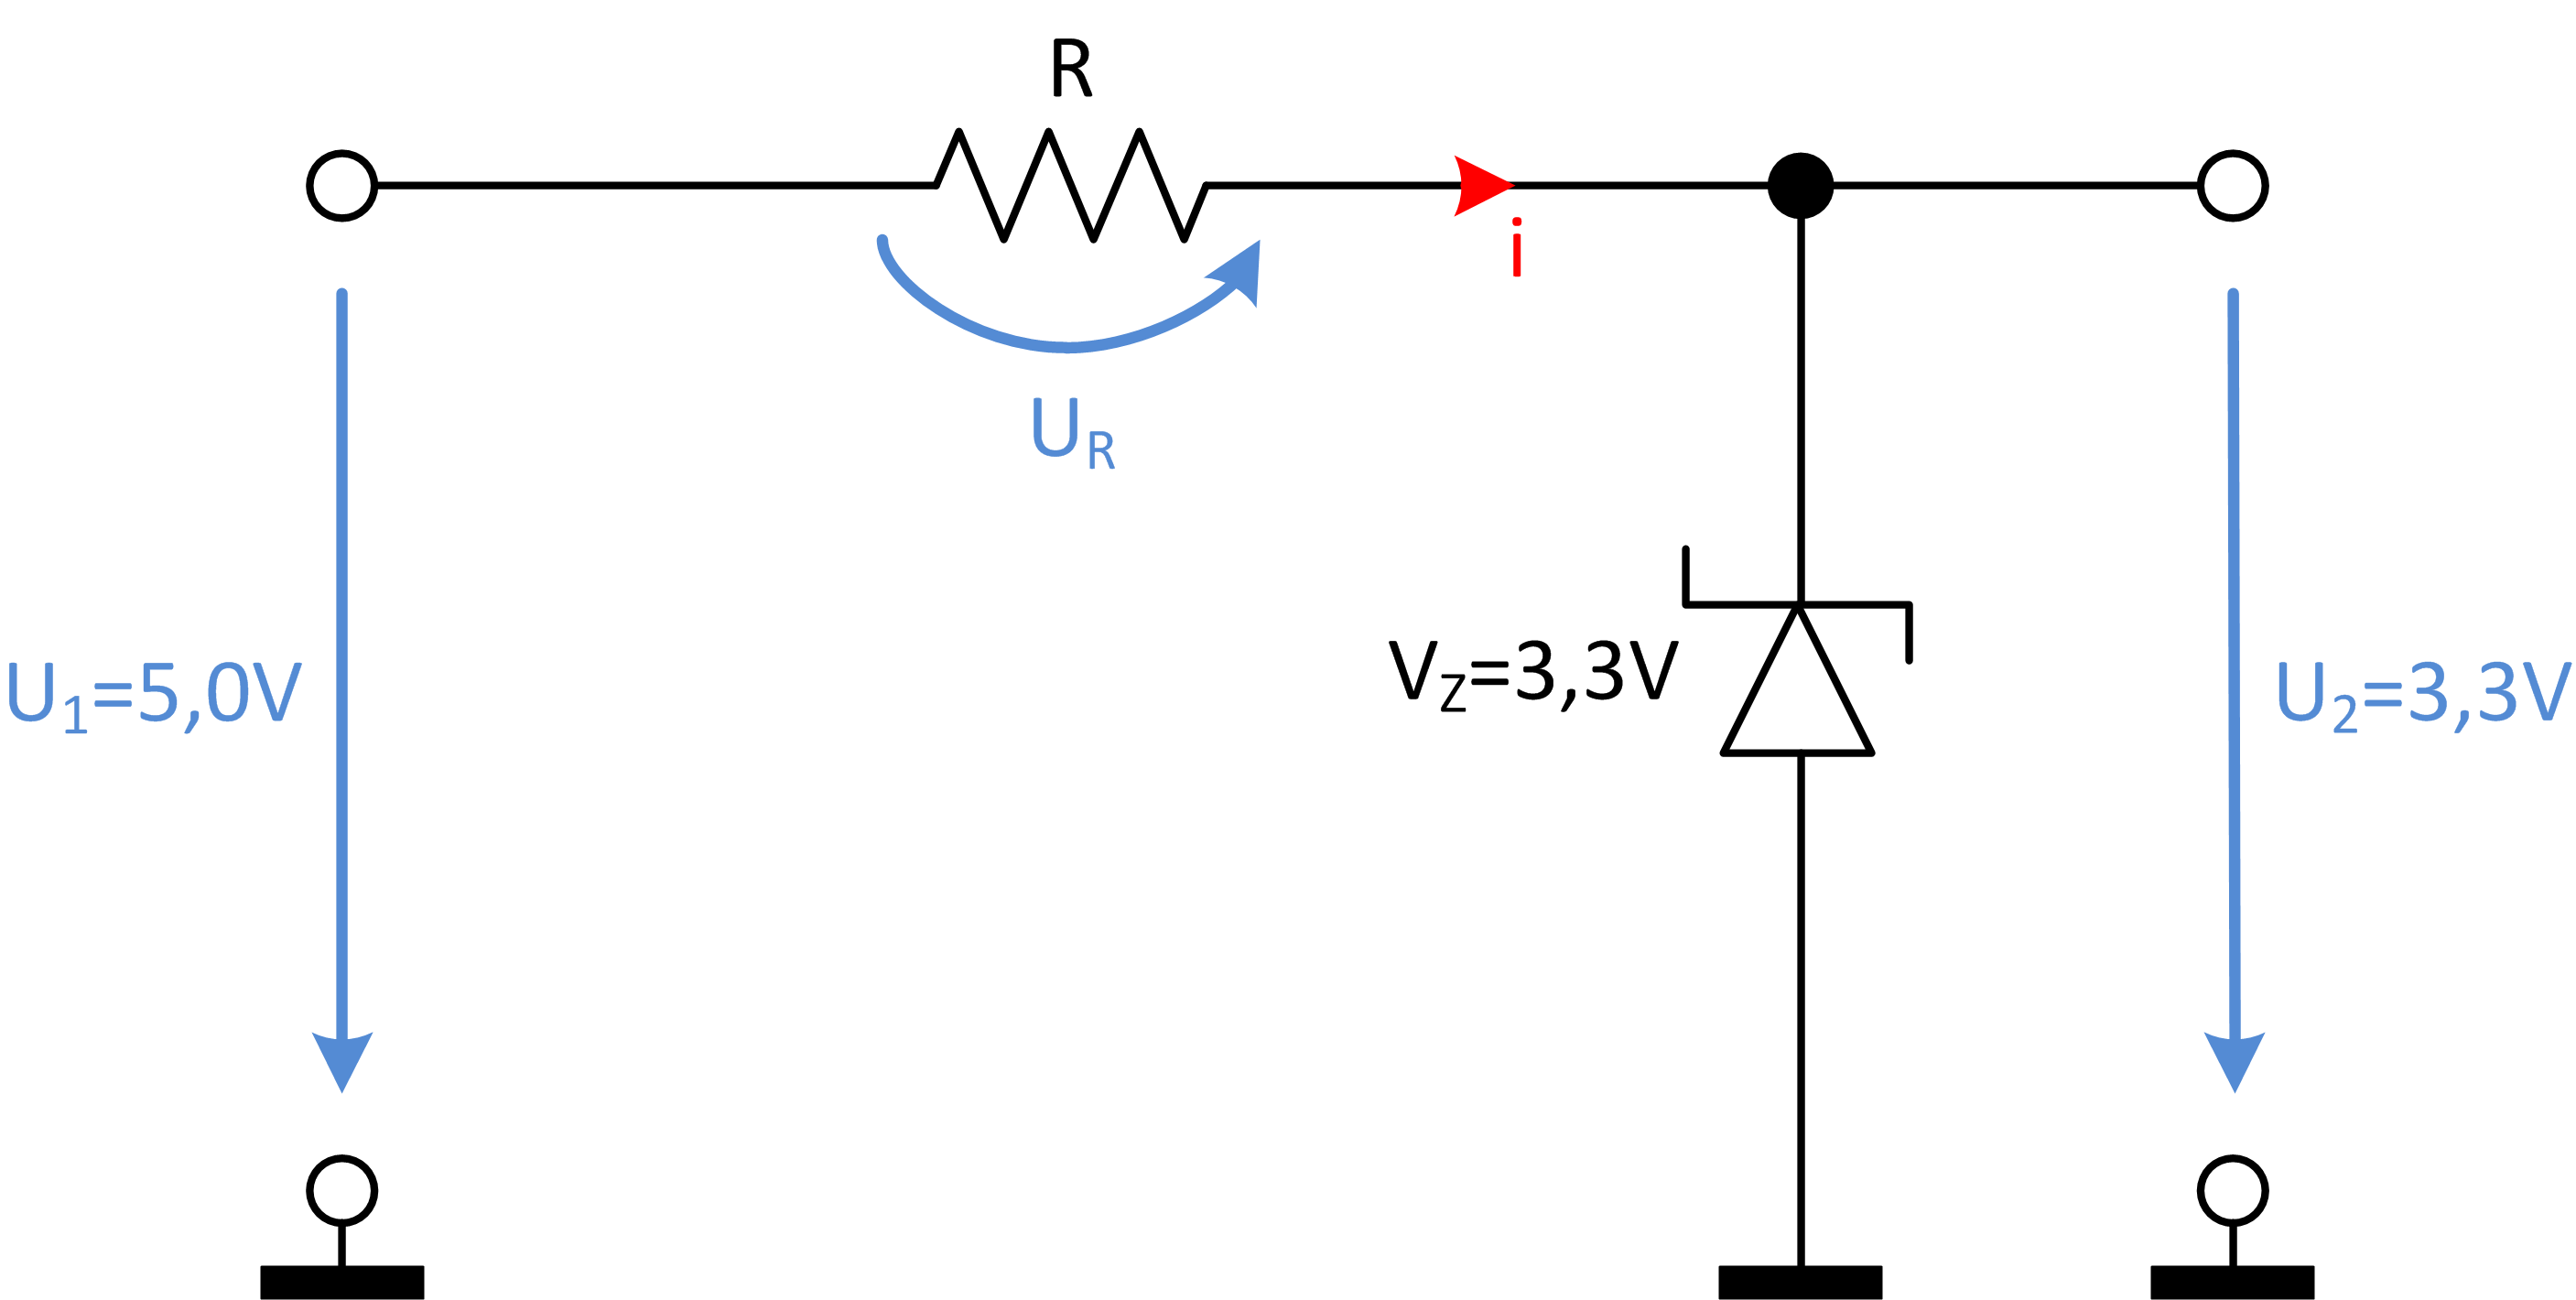
\includegraphics[width=0.60\textwidth]{Beispiel}  
  \caption{Ein Bild als Beispiel}
  \label{fig:beispiel}
\end{center}
\end{figure}
 
Die Positionsdefinition "`htb"' beschreibt die automatische Positionierung in LaTeX in der bevorzugten Reihenfolge "`here, top, buttom"'. Wenn man wei� was man tut und die Grafik in jedem Fall genau an der gew�hlten Stelle eingebunden werden soll ist "`h!"' zu nutzen. Ein Warning\todoedit{zu beachten}\ wird generiert wenn diese Anforderung nicht erf�llt werden kann\todoref{Zu dieser Aussage sollte noch eine Quelle angegeben werden}.
 
\section{Verschiedenes}
\label{sec:haupt:misc}

Ein Beispiel f�r eine nummerierte Tabelle mit Gro�buchstaben und einer speziellen Formatierung:
\begin{enumerate}[\bfseries (A) {-}]
  \item Das Kapitel \ref{sec:haupt} tr�gt den Titel \nameref{sec:haupt}\footnote{Die Nutzung von Nameref ist in vielen Situationen n�tzlich} und beginnt auf Seite \pageref{sec:haupt} 
  \item \SI{3}{\volt} liegt im Bereich zwischen \SIrange[range-units=single]{2,5}{3,5}{\volt}. Die Stromst�rke wird meist in der Einheit \si{\mA} angegeben und auch eine einfache Zahl wie bspw. \num{65536,128} l�sst sich mit dem Package \texttt{siunitx} sicher darstellen.
     
\end{enumerate}


\begin{lstlisting}[caption={\texttt{SCI.c} - SCI-Definitionen}, label=lst:scidefine]
	#define SCIBDH     SCI1BDH
	#define SCIBDL     SCI1BDL
	#define SCIC1      SCI1C1
	#define SCIC2      SCI1C2
	...                ...
\end{lstlisting}

\lstinputlisting[%
		caption=\texttt{wireless\_uart.c} - Auszug,%
		label=lst:scirx,%
		float=hbt,%
		frame={tbrl},%
		%firstline=1,%
		lastline=7,%
]{Sourcecode/bsp.c}

\begin{table}[htb]
\centering
	\begin{tabular}{llr}
	\toprule
	Device & Teiler & Baudrate [Baud]\\
	\midrule
	\multirow{2}{2.5cm}{Modul Standard}
	 & BR=4 & \num{125000}\\
	 & BR=5 & \num{100000}\\
	\cmidrule{2-3}
	& & Diff=\num{25000}\\
	\addlinespace
	\midrule
	\addlinespace
	\multirow{2}{1.5cm}{Modul ExtendedLong}
	 & Step=0x327 & \num{125033}\\
	 & Step=0x326 & \num{124878}\\
	\cmidrule{2-3}
	 & & Diff=\num{155}\\
	\bottomrule
	\end{tabular}
	\caption{Beispiel Tabelle} 
	\label{tab:bsp}
\end{table}
\todoedit{Beachte dasss hier ein Warning wegen dem zu langen Modulnamen erscheint.}





\chapter{Zusammenfassung und Ausblick}

Lorem ipsum dolor sit amet, consetetur sadipscing elitr, sed diam nonumy eirmod tempor invidunt ut labore et dolore magna aliquyam erat, sed diam voluptua. At vero eos et accusam et justo duo dolores et ea rebum. Stet clita kasd gubergren, no sea takimata sanctus est Lorem ipsum dolor sit amet. Lorem ipsum dolor sit amet, consetetur sadipscing elitr, sed diam nonumy eirmod tempor invidunt ut labore et dolore magna aliquyam erat, sed diam voluptua. At vero eos et accusam et justo duo dolores et ea rebum. Stet clita kasd gubergren, no sea takimata sanctus est Lorem ipsum dolor sit amet. Lorem ipsum dolor sit amet, consetetur sadipscing elitr, sed diam nonumy eirmod tempor invidunt ut labore et dolore magna aliquyam erat, sed diam voluptua. At vero eos et accusam et justo duo dolores et ea rebum. Stet clita kasd gubergren, no sea takimata sanctus est Lorem ipsum dolor sit amet.   

Duis autem vel eum iriure dolor in hendrerit in vulputate velit esse molestie consequat, vel illum dolore eu feugiat nulla facilisis at vero eros et accumsan et iusto odio dignissim qui blandit praesent luptatum zzril delenit augue duis dolore te feugait nulla facilisi. Lorem ipsum dolor sit amet, consectetuer adipiscing elit, sed diam nonummy nibh euismod tincidunt ut laoreet dolore magna aliquam erat volutpat.   

Ut wisi enim ad minim veniam, quis nostrud exerci tation ullamcorper suscipit lobortis nisl ut aliquip ex ea commodo consequat. Duis autem vel eum iriure dolor in hendrerit in vulputate velit esse molestie consequat, vel illum dolore eu feugiat nulla facilisis at vero eros et accumsan et iusto odio dignissim qui blandit praesent luptatum zzril delenit augue duis dolore te feugait nulla facilisi.   



%%%%%%%%%%%%%%%%%%%%%%%%%%%%%%%%%%%%%%%%%%%%%%%%%%%%%%%%%%%%%%%%%%%%%%%
%% Anhang und Verzeichnisse
%%%%%%%%%%%%%%%%%%%%%%%%%%%%%%%%%%%%%%%%%%%%%%%%%%%%%%%%%%%%%%%%%%%%%%%
\cleardoublepage

\pagenumbering{Roman}
\begin{appendix}
\chapter{Anhang}

\end{appendix}

\KOMAoptions{open=any}
\addchap{CD-Verzeichnis}
\label{sec:cd}

Dieser Arbeit liegt eine CD bei, \ldots

\markboth{\nomname}{\nomname}
\nocite{*} 					% alle Quellen auff�hren

\printnomenclature			% Abk�rzungsverzeichnis
\listoftables				% Tabellenverzeichnis
\listoffigures				% Abbildungsverzeichnis
\lstlistoflistings			% Listings-Verzeichnis

\KOMAoptions{open=left}		% war in einem Spezialfall sinnvoll
\bibliography{Literatur}	% Literaturverzeichnis
\KOMAoptions{open=right}

\listoftodos				% TODOs, nicht im final Dokument!
%%%%%%%%%%%%%%%%%%%%%%%%%%%%%%%%%%%%%%%%%%%%%%%%%%%%%%%%%%%%%%%%%%%%%%%


%%%%%%%%%%%%%%%%%%%%%%%%%%%%%%%%%%%%%%%%%%%%%%%%%%%%%%%%%%%%%%%%%%%%%%%
%% Eidesstattliche Erkl�rung
%%%%%%%%%%%%%%%%%%%%%%%%%%%%%%%%%%%%%%%%%%%%%%%%%%%%%%%%%%%%%%%%%%%%%%%
\chapter*{Eidesstattliche Erkl�rung}
\thispagestyle{empty}

\vspace{2cm}

\noindent Ich, \autor, Matrikel-Nr.\ \matrikelnr, versichere hiermit, dass ich meine \arbeitsart\ mit dem Thema
\begin{quote}
\textit{\arbeitstitel}
\end{quote}
selbst�ndig verfasst und keine anderen als die angegebenen Quellen und Hilfsmittel benutzt habe, wobei ich alle w�rtlichen und sinngem��en Zitate als solche gekennzeichnet habe. Die Arbeit wurde bisher keiner anderen Pr�fungsbeh�rde vorgelegt und auch nicht ver�ffentlicht.\\[6ex]

\ort, den \today\\

\rule[-0.2cm]{5cm}{0.5pt}

\textsc{\autor}
%%%%%%%%%%%%%%%%%%%%%%%%%%%%%%%%%%%%%%%%%%%%%%%%%%%%%%%%%%%%%%%%%%%%%%%

\end{document}

%%%%%%%%%%%%%%%%%%%%%%%%%%%%%%%%%%%%%%%%%%%%%%%%%%%%%%%%%%%%%%%%%%%%%%%
%% DOKUMENTVORLAGE THOMAS DIETRICH  %%%%%%%%%%%%%%%%%%%%%%%%%%%%%%%%%%%
%%%%%%%%%%%%%%%%%%%%%%%%%%%%%%%%%%%%%%%%%%%%%%%%%%%%%%%%%%%%%%%%%%%%%%%
